\documentclass[aspectratio=169]{ctexbeamer}
%\usetheme{Madrid}
\usetheme{Boadilla}
%\usecolortheme{beaver}
\usepackage{amsmath} 
\usepackage{amssymb} 
\usepackage{amsfonts} 
\usepackage{multicol}
\usepackage{graphicx}
\usepackage{pgfplots}
\pgfplotsset{compat=1.18}
\usefonttheme[onlymath]{serif} % 衬线数学字体

%\setbeamertemplate{theorem}[ams style]
\setbeamertemplate{theorems}[numbered]

\theoremstyle{definition}
\newtheorem{question}{问题}[section]
\newtheorem{exercise}{练习}[section]
\newtheorem{formula}{公式}[section]
\newtheorem{proposition}{命题}[section]
\newtheorem{property}{性质}[section]
	
\title[因式分解]{因式分解}
\subtitle{}
\author[珠海一中创美营]{珠海一中创美营(数学)}
\date[\today]{\today}
%\AtBeginSection[]
%{
%	\begin{frame}
%		\frametitle{目录}
%		\tableofcontents[currentsection]
%	\end{frame}
%}
\begin{document}
\frame{\titlepage}

\section{课程计划}
\begin{frame}{课程计划与参考书籍:小蓝本}
	\begin{multicols}{2}
		数学奥林匹克小丛书·初中卷(第三版),华东师范大学出版社
		\begin{itemize}
			\item 预备知识(因式分解技巧,2次课)
			\item 初等数论(整除、同余和不定方程,10$\sim$12次课)
			\item 平面几何初步(圆,三角形与四边形)
			\item 组合(组合趣题)
			\item 函数与方程(方程与方程组,一次函数与二次函数)
		\end{itemize}
		\begin{figure}
			\flushright
			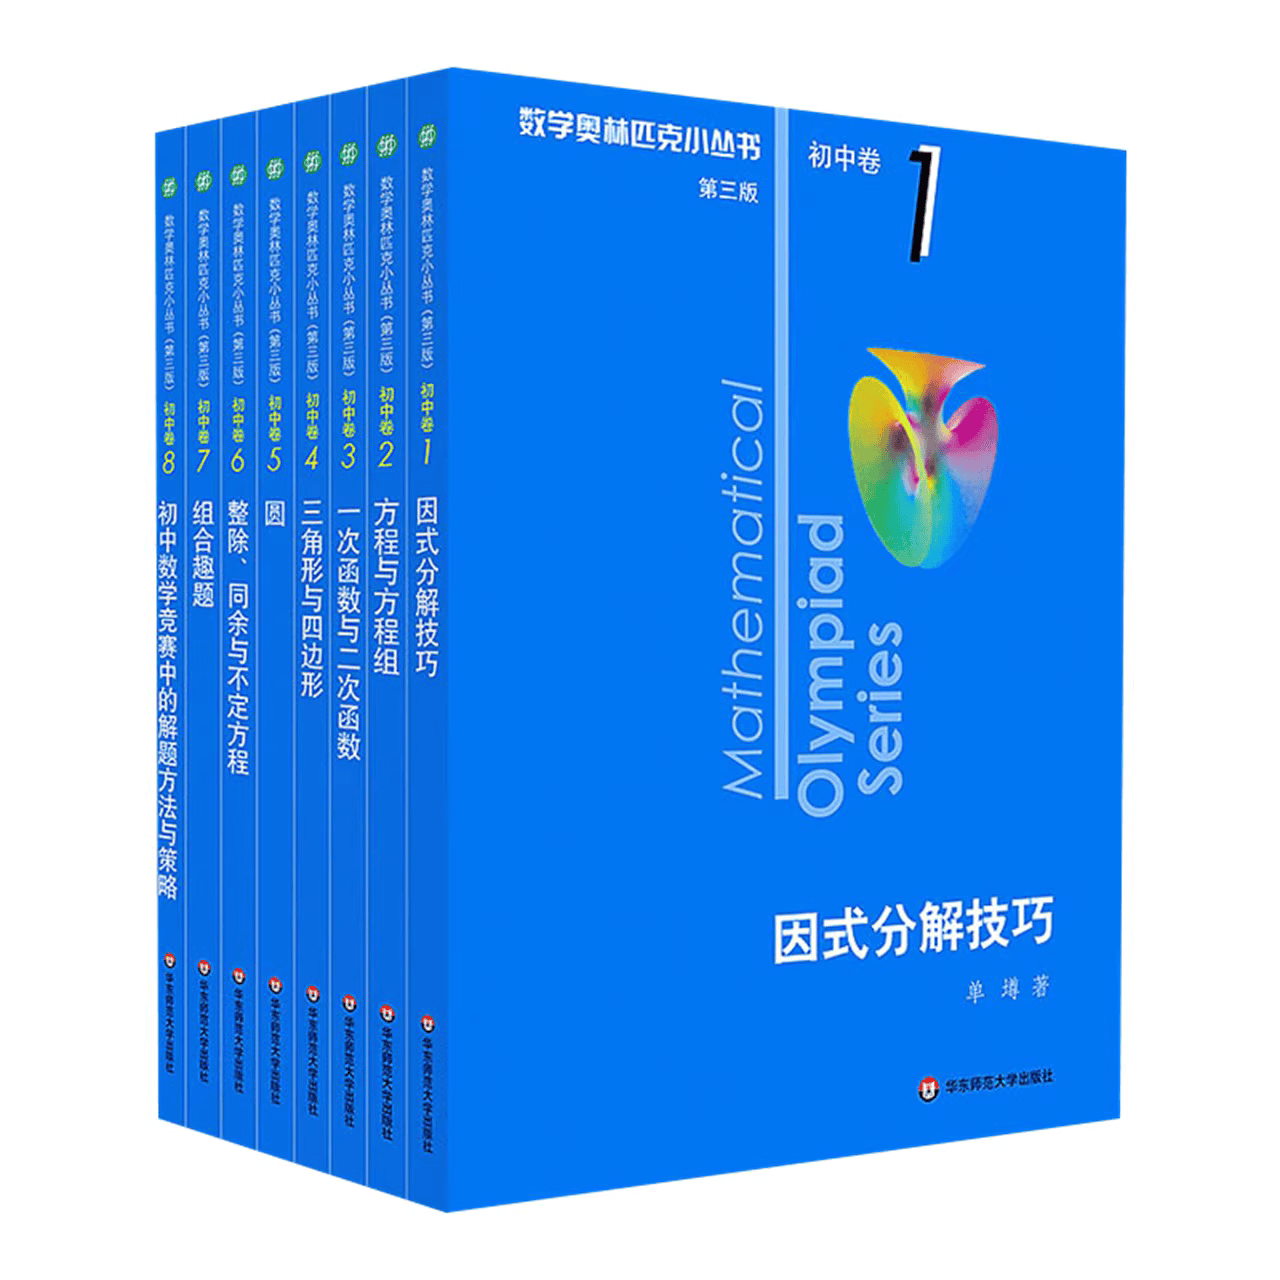
\includegraphics[width=0.4\textwidth]{小蓝本.png}
		\end{figure}
	\end{multicols}
\end{frame}

\begin{frame}{课程要求}
	\begin{itemize}
		\item 上课地点:珠海一中阶梯教室二(尚德楼2栋1楼)
		\item 上课时间:每周六上午8:20-11:20. 50分钟一节课,课间休息10分钟
		\item 每次课前会进行考勤,如需请假提前在群里说明情况
		\item 一中周六在正常自习,课间外出时切勿大声喧哗
		\item 前两节为课堂讲解,最后一节自己做练习,未完成部分留作作业
		\item 8:00由课代表到办公室领取纸质课堂讲义并提前发放,8:20正式开讲
		\item 完整解析版讲义和习题解答会在课后发至QQ群(838572767),课后自行订正习题
		\item 跟上、坚持,遇到不懂的问题多向身边同学和老师提问,觉得简单也不能浅尝辄止,应该对自己有更高的目标和追求
	\end{itemize}
\end{frame}

\begin{frame}{课程目标}
	培养珠海一中五大学科竞赛的预备军,为进入创美班(竞赛班)做好准备,争取省一以及更高的奖项(省队、国集)
\end{frame}

\section{提公因式}
% 例 1
\begin{frame}[t]{提公因式}
	\begin{example}[一次提净]\label{ex:提公因式-例1-一次提净}
		分解因式: $12 a^{2} x^{3}+6 a b x^{2} y-15 a c x^{2}$
	\end{example}
\end{frame}

% 例 2
\begin{frame}[t]
	\begin{example}[视“多”为一]\label{ex:提公因式-例2-一次提净}
		分解因式: $2 a^{2} b(x+y)^{2}(b+c)-6 a^{3} b^{3}(x+y)(b+c)^{2}$
	\end{example}
\end{frame}

% 例 3
\begin{frame}[t]
	\begin{example}[切勿漏 1]
		分解因式: $(2 x+y)^{3}-(2 x+y)^{2}+(2 x+y)$.
	\end{example}
\end{frame}

% 例 4
\begin{frame}[t]
	\begin{example}[注意符号]\label{ex:提公因式-例4-注意符号}
		分解因式: $-3 a b(2 x+3 y)^{4}+a c(2 x+3 y)^{3}-a(2 x+3 y)$.
	\end{example}
\end{frame}

% 例 5
\begin{frame}[t]
	\begin{example}[仔细观察]\label{ex:提公因式-例5-仔细观察}
		分解因式: $(2 x-3 y)(3 x-2 y)+(2 y-3 x)(2 x+3 y)$ .
	\end{example}
\end{frame}

% 例 6
\begin{frame}[t]
	\begin{example}[化“分”为整]\label{ex:提公因式-例6-化分为整}
		分解因式: $3 a^{3} b^{2}-6 a^{2} b^{3}+\frac{27}{4} a b$.
	\end{example}
\end{frame}

\section{应用公式}
\begin{frame}{应用公式}
	\begin{enumerate}
		\item $a^{2}-b^{2}=(a+b)(a-b)$.
		\item $a^{3}+b^{3}=(a+b)\left(a^{2}-a b+b^{2}\right)$.
		\item $a^{3}-b^{3}=(a-b)\left(a^{2}+a b+b^{2}\right)$.
		\item $a^{2}+2 a b+b^{2}=(a+b)^{2}$.
		\item $a^{2}-2 a b+b^{2}=(a-b)^{2}$.
		\item $a^{3}+3 a^{2} b+3 a b^{2}+b^{3}=(a+b)^{3}$.
		\item $a^{3}-3 a^{2} b+3 a b^{2}-b^{3}=(a-b)^{3}$.
	\end{enumerate}
\end{frame}

\setcounter{theorem}{0}
% 例 1
\begin{frame}[t]{平方差}
	\begin{example}
		分解因式: $9(m-n)^{2}-4(m+n)^{2}$ .
	\end{example}
\end{frame}

% ·例 2
\begin{frame}[t]{平方差}
	\begin{example}
		分解因式: $75 x^{6} y-12 x^{2} y^{5}$.
	\end{example}
\end{frame}

% 例 3
\begin{frame}[t]{平方差}
	\begin{example}\label{ex:应用公式-例3}
		分解因式: $-\left(3 a^{2}-5 b^{2}\right)^{2}+\left(5 a^{2}-3 b^{2}\right)^{2}$.
	\end{example}
\end{frame}


% 例 4
\begin{frame}[t]{立方和与立方差}
	\begin{example}
		分解因式: $9 x^{5}-72 x^{2} y^{3}$ .
	\end{example}
\end{frame}

% 例 5
\begin{frame}[t]{立方和与立方差}
	\begin{example}
		分解因式: $a^{6}+b^{6}$ .
	\end{example}
\end{frame}

% 例 6
\begin{frame}[t]{完全平方}
	\begin{example}
		分解因式: $9 x^{2}-24 x y+16 y^{2}$ .
	\end{example}
\end{frame}

% 例 7
\begin{frame}[t]{完全平方}
	\begin{example}
		分解因式: $8 a-4 a^{2}-4$ .
	\end{example}
\end{frame}

% 例 8
\begin{frame}[t]{完全平方}
	\begin{example}\label{ex:应用公式-例8}
		分解因式: $4 a^{2}+9 b^{2}+9 c^{2}-18 b c-12 c a+12 a b$ .
	\end{example}
\end{frame}

% 例 9
\begin{frame}[t]{完全立方}
	\begin{example}
		分解因式: $8 x^{3}+27 y^{3}+36 x^{2} y+54 x y^{2}$ .
	\end{example}
\end{frame}

% 例 10
\begin{frame}[t]{完全立方}
	\begin{example}
		分解因式: $729 a^{6}-243 a^{4}+27 a^{2}-1$.
	\end{example}
\end{frame}

% 例 11
\begin{frame}[t]{举一反三}
	\begin{example}
		分解因式: $a^{6}-b^{6}$ .
	\end{example}
\end{frame}

% 例 12
\begin{frame}[t]{高阶运用}
	\begin{example}
		求证 $2^{1984}+1$ 不是质数.
	\end{example}
\end{frame}

% 例 13
\begin{frame}[t]
	\begin{example}
		分解因式: $x^{5}-1$.
	\end{example}
\end{frame}

\section*{未完待续}
\begin{frame}
	\Huge
	$$
		\mathcal{TO}	\quad
		\mathcal{BE}  	\quad
		\mathcal{CONTINUED}
		\ldots
	$$
\end{frame}
\end{document}

